% Ecosystem data flow - directed acyclic graph of the repository handoffs.
% Replaces the monospace block on docs/intro/03_ecosystem.rst.
\documentclass[border=3mm]{standalone}
\usepackage{tikz}
\usetikzlibrary{arrows.meta, positioning, calc}
\usepackage[T1]{fontenc}
\usepackage{lmodern}

\definecolor{IHPfg}{RGB}{0,80,139}
\definecolor{IHPaccent}{RGB}{109,112,114}
\definecolor{IHPgreen}{RGB}{65,155,75}
\definecolor{cGDS2K}{RGB}{228,15,19}
\definecolor{cPDK}{RGB}{190,125,35}
\definecolor{cKicad}{RGB}{0,80,139}
\definecolor{cChiplet}{RGB}{55,145,195}
\definecolor{cDesigns}{RGB}{120,70,150}

\begin{document}
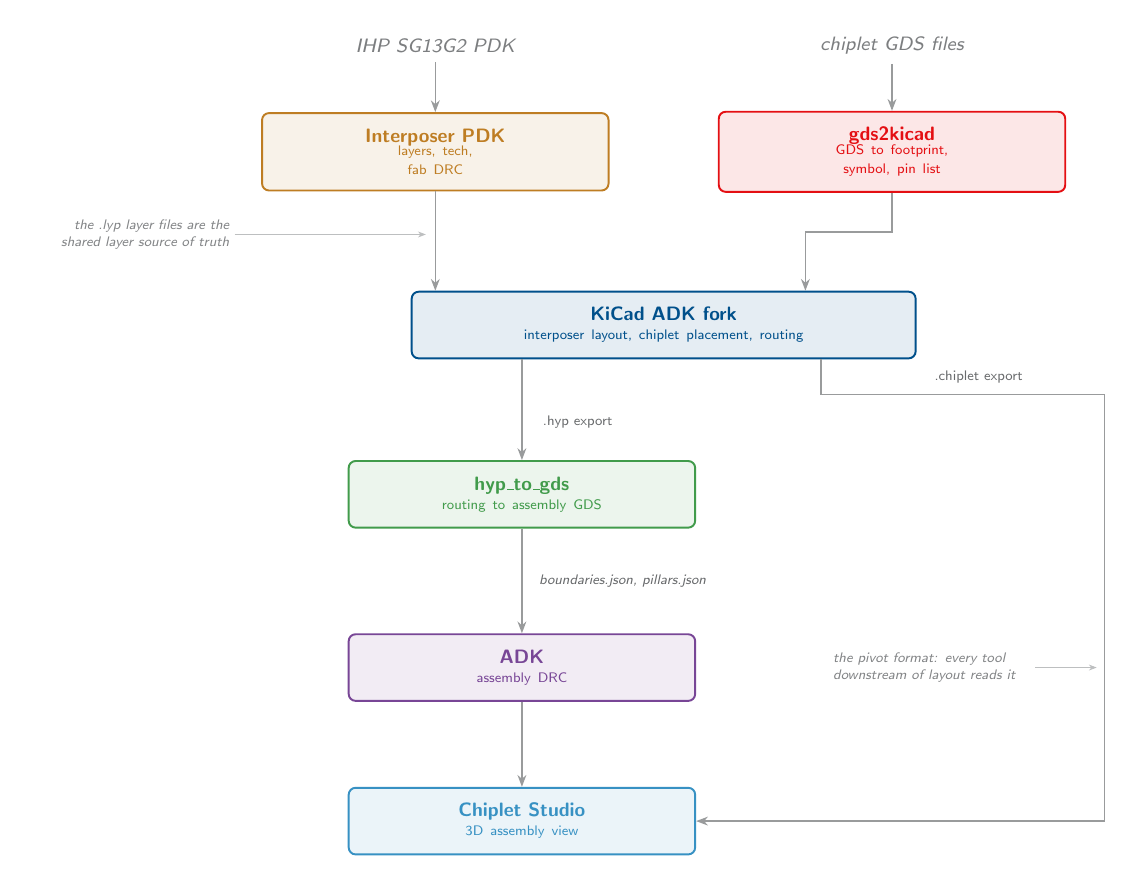
\begin{tikzpicture}[
    >=Stealth,
    adkbox/.style={
        rectangle, rounded corners=2.5pt,
        draw=#1, fill=#1!10, line width=0.7pt,
        text width=40mm, inner sep=2mm,
        font=\sffamily\scriptsize, text=#1, align=center
    },
    adkwide/.style={
        rectangle, rounded corners=2.5pt,
        draw=#1, fill=#1!10, line width=0.7pt,
        text width=60mm, inner sep=2mm,
        font=\sffamily\scriptsize, text=#1, align=center
    },
    adksrc/.style={
        font=\sffamily\scriptsize\itshape, text=IHPaccent!90, align=center
    },
    adkarrow/.style={
        -{Stealth[length=1.5mm]}, line width=0.5pt, color=IHPaccent!70
    },
    adkedgelbl/.style={
        font=\sffamily\tiny, text=IHPaccent!95!black, inner sep=0.6mm
    },
    adkannot/.style={
        font=\sffamily\tiny\itshape, text=IHPaccent!85,
        text width=25mm, inner sep=0.6mm
    },
    adklead/.style={
        -{Stealth[length=1mm]}, line width=0.3pt, color=IHPaccent!45
    }
]

% =================================================================== nodes

% rank 0, two sources, no box
\node[adksrc] (srcpdk) at (-2.9, 6.55) {IHP SG13G2 PDK};
\node[adksrc] (srcgds) at ( 2.9, 6.55) {chiplet GDS files};

% rank 1
\node[adkbox=cPDK] (ipdk) at (-2.9, 5.20)
    {\textbf{Interposer PDK}\\[-0.4mm]{\tiny layers, tech,\\[-0.4mm]fab DRC}};

\node[adkbox=cGDS2K] (g2k) at ( 2.9, 5.20)
    {\textbf{gds2kicad}\\[-0.4mm]{\tiny GDS to footprint,\\[-0.4mm]symbol, pin list}};

% rank 2
\node[adkwide=cKicad] (kicad) at (0, 3.00)
    {\textbf{KiCad ADK fork}\\[-0.4mm]{\tiny interposer layout, chiplet placement, routing}};

% rank 3
\node[adkbox=IHPgreen] (hyp) at (-1.8, 0.85)
    {\textbf{hyp\_to\_gds}\\[-0.4mm]{\tiny routing to assembly GDS}};

% rank 4
\node[adkbox=cDesigns] (adk) at (-1.8, -1.35)
    {\textbf{ADK}\\[-0.4mm]{\tiny assembly DRC}};

% rank 5, sink
\node[adkbox=cChiplet] (studio) at (-1.8, -3.30)
    {\textbf{Chiplet Studio}\\[-0.4mm]{\tiny 3D assembly view}};

% =================================================================== edges

% sources into rank 1
\draw[adkarrow] (srcpdk.south) -- (ipdk.north);
\draw[adkarrow] (srcgds.south) -- (g2k.north);

% rank 1 into rank 2
\draw[adkarrow] (ipdk.south) -- (ipdk.south |- kicad.north);
\draw[adkarrow] (g2k.south) -- ++(0,-0.50) -| ([xshift=18mm]kicad.north);

% rank 2 out, left branch
\draw[adkarrow] ([xshift=-18mm]kicad.south)
    -- ([xshift=-18mm]kicad.south |- hyp.north);
\node[adkedgelbl, anchor=west] at ([xshift=-16mm, yshift=-8mm]kicad.south)
    {.hyp export};

% rank 2 out, right branch: the .chiplet edge bypasses the DRC path
\coordinate (cA) at ([xshift=20mm, yshift=-4.5mm]kicad.south);
\coordinate (cB) at ($(cA)+(3.6,0)$);
\draw[adkarrow] ([xshift=20mm]kicad.south) -- (cA) -- (cB)
    -- (cB |- studio.east) -- (studio.east);
\node[adkedgelbl, anchor=south] at ([xshift=-16mm, yshift=0.8mm]cB)
    {.chiplet export};

% rank 3 into rank 4
\draw[adkarrow] (hyp.south) -- (adk.north);
\node[adkedgelbl, anchor=west, font=\sffamily\tiny\itshape] at (-1.65, -0.25)
    {boundaries.json, pillars.json};

% rank 4 into the sink
\draw[adkarrow] (adk.south) -- (studio.north);

% =============================================================== callouts

\node[adkannot, anchor=east] (noteA) at (4.72, -1.35)
    {the pivot format: every tool downstream of layout reads it};
\draw[adklead] (noteA.east) -- (5.50, -1.35);

\node[adkannot, anchor=east, align=right] (noteB) at (-5.45, 4.15)
    {the .lyp layer files are the shared layer source of truth};
\draw[adklead] (noteB.east) -- (-3.02, 4.15);

\end{tikzpicture}
\end{document}
